\documentclass[../../thesis.tex]{subfiles}

\begin{document}
\begin{figure}[tb]
    \centering
    \pgfdeclarelayer{bg}    % declare background layer
    \pgfsetlayers{bg,main}  % set the order of the layers (main is the standard layer)
    \subfloat[]{
      \tikzsetnextfilename{etch_rate_plot}
      \begin{tikzpicture}
          \begin{axis}[
            /tikz/line join=bevel,
            width=0.25*\textwidth,
            height=0.25*\textwidth,
            legend style={at={(0,.5)}, legend columns=1, anchor=south west},
            every axis plot,
  					line width = 1pt,
  					xmin = 0, xmax = 60,
  					ymin = 0, ymax = 6/13,
  					xlabel = {Height within the pores $h$ in $\si{\micro\meter}$},
  					ylabel = {Etch rate $e_\mathrm{\perp pores}$ in $\si{\nano\meter\per\minute}$},
            grid
            ]
  					% Add plots
            \addplot [color=red, mark=none]
              coordinates {
              (0, 6/13)
              (60,0)};
          \end{axis}
      \end{tikzpicture}
      \label{fig:etch_rate_plot}
    }
    \hfill
    \subfloat[]{
      \tikzsetnextfilename{funnelling_increase}
      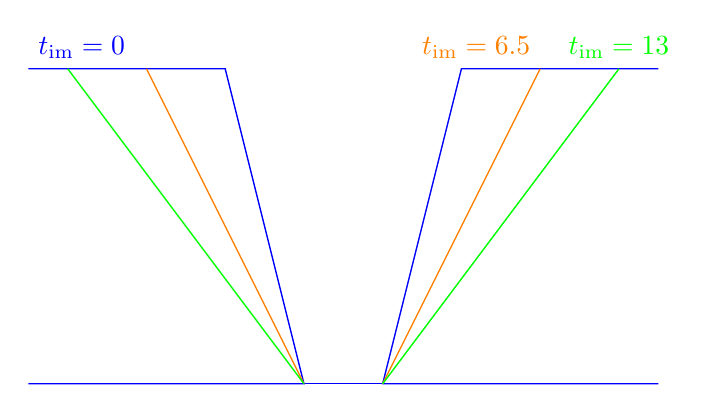
\begin{tikzpicture}
          \draw[line width=0.5,color=blue] (0.5,0)--(4,0)--(3,4)--(0.5,4) node[anchor=south west] {$t_\mathrm{im}=\SI{0}{\minute}$};
          \draw[line width=0.5,color=blue] (8.5,0)--(5,0)--(6,4)--(8.5,4);
          \draw[line width=0.5,color=blue] (4,0)--(5,0);
          \draw[line width=0.5,color=orange] (4,0)--(2,4);
          \draw[line width=0.5,color=orange] (5,0)--(7,4) node[anchor=south east] {$t_\mathrm{im}=\SI{6.5}{\minute}$};
          \draw[line width=0.5,color=green] (4,0)--(1,4);
          \draw[line width=0.5,color=green] (5,0)--(8,4) node[anchor=south] {$t_\mathrm{im}=\SI{13}{\minute}$};
      \end{tikzpicture}
      \label{fig:funneling_increase}
    }
    \caption{Immersion of a closed pore membrane resulting in an increase of the funnelling aspect of the pores as shown in \protect\subref{fig:funneling_increase} due to the saturation of the acid within the pores. The visualized theory is backed by the isotherms in \cref{fig:immersed-comp-w296} which lead to the etch rate dependency plotted in \protect\subref{fig:etch_rate_plot} on the height within a pore. For further explanations please refer to \cref{subsec:immersed-membranes}.}
\end{figure}
\end{document}
